\chapter{Casi d'suo}
I casi d'uso permettono di modellare il comportamento del sistema e descrivere i requisiti funzionali in linguaggio naturale. Grazie a questi modelli è quindi possibile rappresentare il comportamento esterno del sistema, visto come una black-box, dal punto di vista di un attore.

Oltre a una descrizione testuale (gli \emph{Scenari}) i casi d'uso possono esser rappresentati mediante diagrammi. In tali diagrammi troviamo le segunti entità:
 \begin{itemize}
  \item gli attori: essi rappresentano un soggetto o un'entità esterna che interagisce col sistema
  \item i casi d'uso: rappresentano un particolare scenario di interazione tra attore e sistema. Sono rappresentati graficamente da ellissi
  \item le associazioni: rappresentate da una linea mettono in comunicazione un attore con i caso d'uso
 \end{itemize}

 Nei prossimi paragrafi saranno mostrati alcuni dei casi d'uso modellati durante la fase di analisi.
 \section{Diagrammi dei casi d'uso}
 \subsection{Caso d'uso 1\_0 Ricarica telefonica}
	\begin{figure}[!htbp]
	  \centering
	  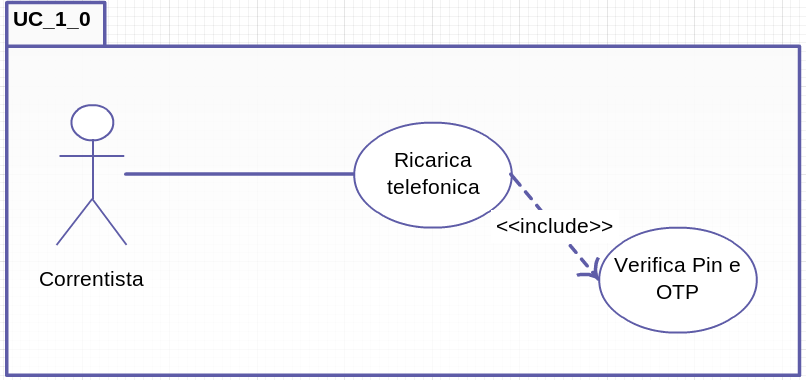
\includegraphics[scale=0.50]{casi_uso/ricarica.png}
	\end{figure}
 
 
 \section{Specifica dei casi d'uso}
 \subsection{Caso d'uso 1\_0 Ricarica telefonica}

\begin{center}
     \begin{longtable}{{ | l | p{8cm} |}}
    \hline
    \textbf{Caso d'uso} & Ricarica telefonica di un numero salvato in rubrica \\ \hline
    \textbf{Attore} & Correntista bancario  \\ \hline
    \textbf{Precondizioni} & L'utente è loggato al sistema e ha iniziato una sessione inserendo un codice OTP  \\ \hline
    \textbf{Postcondizioni di successo}  & Il sistema ha registrato l'operazione \\\hline
    \textbf{Postcondizioni di fallimento}   &  Il sistema non ha registrato l'operazione\\\hline
    \textbf{Scenario} &  \\\hline
    & \begin{enumerate}
       \item L'utente seleziona l'operazione di ricarica telefonica
       \item \label{item:sel1}Il sistema visualizza l'elenco dei beneficiari
       \item L'utente seleziona un beneficiario 
       \item \label{item:sel2}Il sistema visualizza l'elenco dei conti per l'addebbito
       \item L'utente seleziona un conto
       \item \label{item:sel3}\label{item:compagnia} Il sistema mostra l'elenco delle compagnie telefoniche
       \item L'utente seleziona una compagnia telefonica
       \item \label{item:sel4}Il sistema visualizza i tagli disponibili
       \item L'utente seleziona un taglio di ricarica
       \item \label{item:sel5}\label{item:beneficiario} Il sistema mostra il riepilogo dell'operazione e richiede conferma
       \item L'utente conferma i dati
       \item \label{item:credenziali}\label{item:sel6}Il sistema richiede Pin e OTP
       \item L'utente immette i dati richiesti e conferma
       \item \texttt{Include} \emph{Verifica credenziali}
       \item Il sistema mostra lo scontrino dell'operazione
      \end{enumerate}\\\hline
      \textbf{Scenari alternativi} &  \\\hline
    & \begin{enumerate}
    \setcounter{enumi}{2}
       \item L'utente seleziona la voce \emph{beneficiario}
       \item Il sistema mostra la lista beneficiari
       \item L'utente seleziona il beneficiario
       \item Il caso d'uso riprende dal punto \ref{item:beneficiario}
      \end{enumerate}\\\hline
     & \begin{itemize}
       \item  \ref{item:sel1}, \ref{item:sel2}, \ref{item:sel3}, \ref{item:sel4}, \ref{item:sel5}, \ref{item:sel6} L'utente annulla operazione
       \item Il caso d'uso termina
      \end{itemize}\\\hline
    \textbf{Scenari di errore} &  \\\hline
    & \begin{enumerate}
    \setcounter{enumi}{6}
       \item L'utente seleziona una compagnia telefonica errata
       \item Il sistema mostra messaggio di errore
       \item Il caso d'uso riprende dal punto \ref{item:compagnia}
      \end{enumerate}\\\hline
           & \begin{enumerate}
    \setcounter{enumi}{13}
       \item Il sistema non valida le credenziali
       \item Il sistema comunica tipo di errore
       \item Il caso d'uso riprende dal punto \ref{item:credenziali}
      \end{enumerate}\\\hline

     \end{longtable}
\end{center}

\subsection{Caso d'uso 2\_0 Consultare lista conti e carte}

\begin{center}
     \begin{longtable}{{ | l | p{8cm} |}}
    \hline
    \textbf{Caso d'uso} &  Consultare lista conti e carte \\ \hline
    \textbf{Attore} & Correntista bancario  \\ \hline
    \textbf{Precondizioni} & L'utente è loggato al sistema e o ha attivato \emph{ricorda credenziali}  \\ \hline
    \textbf{Postcondizioni di successo}  & Il sistema rimane nel suo stato o aggiorna la lista dei conti in memoria \\\hline
    \textbf{Postcondizioni di fallimento}   &  Il sistema rimane nel suo stato\\\hline
    \textbf{Scenario} &  \\\hline
    & \begin{enumerate}
       \item L'utente seleziona l'operazione di visualizzazione lista conti e carte
       \item \label{item:verificalista}Il sistema verifica che l'elenco dei prodotti non è vuoto
       \item \label{item:sel1}Il sistema mostra la lista dei prodotti
       \item \texttt{Extend} \emph{Visualizza lista movimenti}
      \end{enumerate}\\\hline
    \textbf{Scenario alternativo} &  \\\hline
    & \begin{enumerate}
    \setcounter{enumi}{1}
       \item Il sistema verifica che la lista dei prodotti è vuota
       \item Il sistema notifica l'evento con un opportuno messaggio
	\item Il caso d'uso termina
       \end{enumerate}\\\hline
    \textbf{Scenario di errore} &  \\\hline
    & \begin{enumerate}
    \setcounter{enumi}{1}
       \item Il sistema riceve un errore
       \item Il sistema notifica l'evento con un messaggio di errore e la possibilità di riprovare l'azione
       \item L'utente seleziona \emph{riprova}
       \item Il caso d'uso riprende dal punto \ref{item:verificalista}
       \end{enumerate}\\\hline
     \end{longtable}
\end{center}
